\chapter[Klasifikácia]{Klasifikácia na základe lokálnej informácie}

\section{Úloha klasifikátora}

V našej práci sme klasifikátor použili na zakomponovaní dodatočných informácií o sekvenciách do modelu zarovnania sekvencií. Dodatočné informácie sú poskytnuté formou anotácií k príslušným bázam.

V našich modeloch sme použili 2 typy klasifikátorov -- \textit{Match klasifikátor} a \textit{InDel klasifikátor}.

Match klasifikátor sa klasifikátor určuje s akou pravdepodobnosťou sa majú dané dve pozície v sekvenciách zarovnať k sebe. Jeho výstupom je číslo z intervalu $\left<0,1\right>$, pričom čím bližšie je toto čislo k 1, tým si je klasifikátor istejší, že dané 2 pozície sa majú zarovnať k sebe. Naopak, čím bližšie je k 0, tým si je viac istý, že by tieto pozície k sebe byť nemajú.

InDel klasifikátor urcuje s akou pravdepodobnosťou má byť pozícia v príslušnej sekvencii zarovnaná s medzerou. Jeho výstupom je opäť  číslo z intervalu $\left<0,1\right>$, pričom čím bližšie je toto čislo k 1, tým si je klasifikátor istejší, že daná pozícia sa má zarovnať k medzere a čím bližšie je k 0, tým si je viac istý, že sa táto pozícia nemá zarovnať k medzere.

Tieto pravdepodobnosti sú akousi mierou istoty daného klasifikátora, a keďže tieto 2 klasifikátory sú nezávislé, súčet ich výstupov nemusí byť jedna.

\section{Vstupné dáta}

V práci sme vyskúšali a porovnali viacero typov vstupných dát a porovnali sme ako dobre sa klasifikátor na týchto dátach učí. Všetky typy dát sú založené na okne okolo daných pozícií, ktoré je definované v nasledujúcej sekcii.

Na porovnanie typov dát sme používali dve miery -- dôležitosť atribútov a úspešnosť klasifikátora.

\subsection{Definícia okna}
\label{subsec:window}
Ako vstupné dáta dostane klasifikátor okolie okolo daných pozícií. Toto okolie budeme volať \textit{okno}. Okno veľkosti $w$ pozostáva z $2w$ blokov veľkosti $k = (1+\#\text{anotácií})$.

Majme teda dve sekvencie, $X = x_1 x_2 \dots x_n$ a $Y = y_1 y_2 \dots y_n$ a pozície $i$ a $j$.
Pri Match klasifikátore okno veľkosti $w$ obsahuje $x_{i - w/2}\dots x_i \dots x_{i + (1 + w)/2}$, $y_{j - w/2}\dots y_j \dots y_{j + (1 + w)/2}$ a všetky anotácie príslušných báz. (Obr. \ref{fig:window-m})

Pri InDel klasifikátore používame tiež dve pozície -- prvá je pozícia v inzert sekvencii a ukazuje na bázu, na ktorú sa pýtame a druhá pozícia je v druhej sekvencii a ukazuje na medzeru, teda medzi dve bázy.
Predpokladajme teraz, že $X$ je inzert sekvencia. Okno Indel klasifikátora veľkosti $w$ obsahuje $x_{i - w/2}\dots x_i \dots x_{i + (1 + w)/2}$, $y_{j - w/2}\dots y_j \dots y_{j + (1 + w)/2 - 1}$ a všetky anotácie príslušných báz. (Obr. \ref{fig:window-i})

\begin{figure}[h]
        \centering
        \begin{subfigure}[b]{0.35\textwidth}
                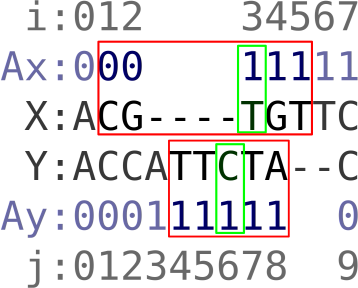
\includegraphics[width=\textwidth]{images/window_m}
                \caption{Match klasifikátor}
                \label{fig:window-m}
        \end{subfigure}%
        \qquad\qquad %add desired spacing between images, e. g. ~, \quad, \qquad etc.
          %(or a blank line to force the subfigure onto a new line)
        \begin{subfigure}[b]{0.35\textwidth}
                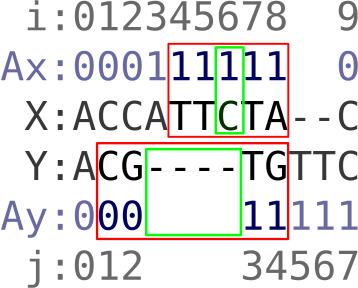
\includegraphics[width=\textwidth]{images/window_i}
                \caption{InDel klasifikátor}
                \label{fig:window-i}
        \end{subfigure}
        \caption[Okno klasifikátora]{Okno klasifikátora pre pozície $i = 6$ a $j = 3$}
\end{figure}


\subsection{Typ dát č. 1 - okno bez úpravy}
\label{subsec:datatype1}

Ako prvý typ dát sme zobrali okno tak ako sme ho definovali v predošlej sekcii (\ref{subsec:window}). Dáta obsahujú priamo všetky bázy a anotácie tak ako sú v okne.

Na obrázku \ref{fig:datatype1-m} si móžme všimnút, že Match klasifikátor sa zameral najmä na bázy a anotácie skoro nebral do úvahy.
Toto správanie zodpovedá tomu, že v praxi bázy majú podstatne väčší význam pri zarovnávaní sekvencií.
Je dôležité si tiež všimnúť veľké odchýlky pri jednotlivých klasifikátoroch. To poukazuje na veľkú rôznorodosť jednotlivých klasifikátorov.

Indel klasifikátor sa podľa obrázku \ref{fig:datatype1-i} tiež zameral hlavne na bázy a to hlavne na strednú bázu $x$-ovej sekvencie a 3-tiu bázu $y$-ovej sekvencie. Dôvodom sú hlavne negatívne príklady pri trénovaní, ktoré zodpovedajú zarovnaným pozíciám, a v nich sú tieto pozície často zhodné a teda v tom prípade by klasifikátor mal vracať hodnoty blízke 0.

\begin{figure}[htp]
        \centering
        \begin{subfigure}[t]{0.4\textwidth}
                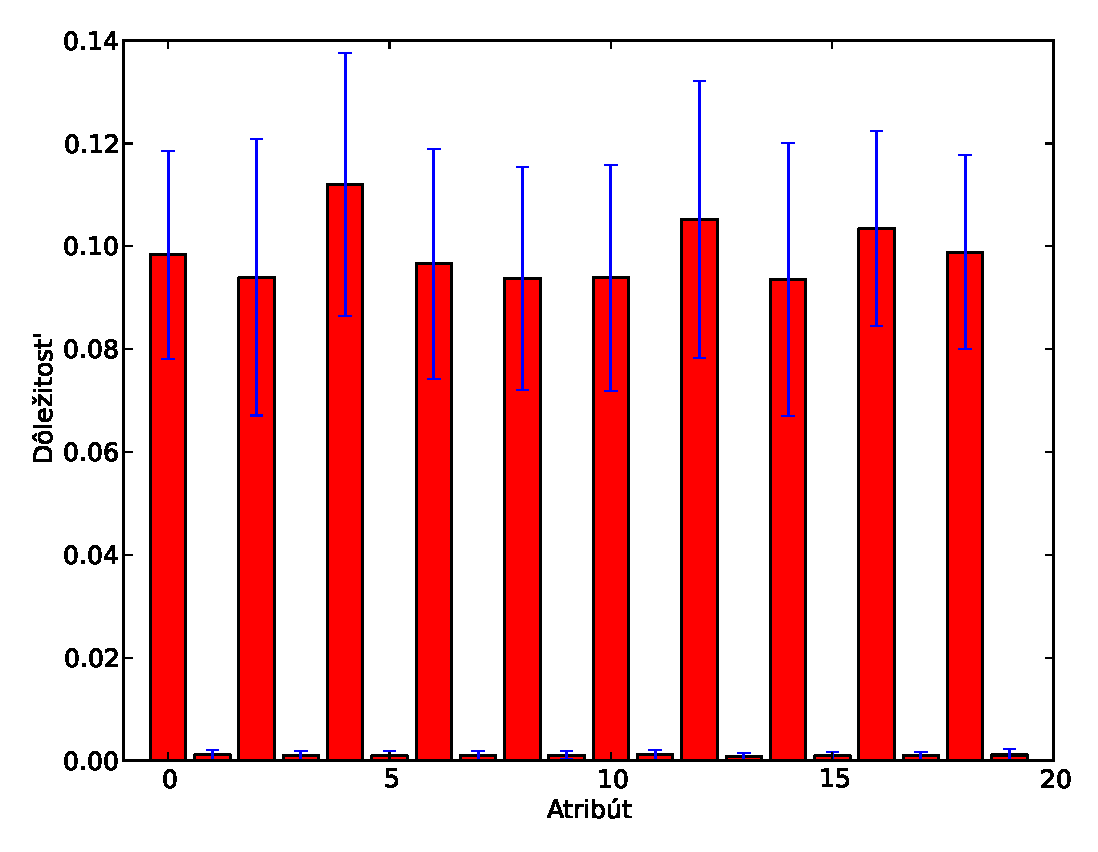
\includegraphics[width=\textwidth]{images/clf_fi/randomforest5_bars}
                \includegraphics[width=\textwidth]{images/clf_fi/randomforest5_heatmap}
                \caption{Match klasifikátor}
                \label{fig:datatype1-m}
        \end{subfigure}%
        \qquad\qquad %add desired spacing between images, e. g. ~, \quad, \qquad etc.
          %(or a blank line to force the subfigure onto a new line)
        \begin{subfigure}[t]{0.4\textwidth}
                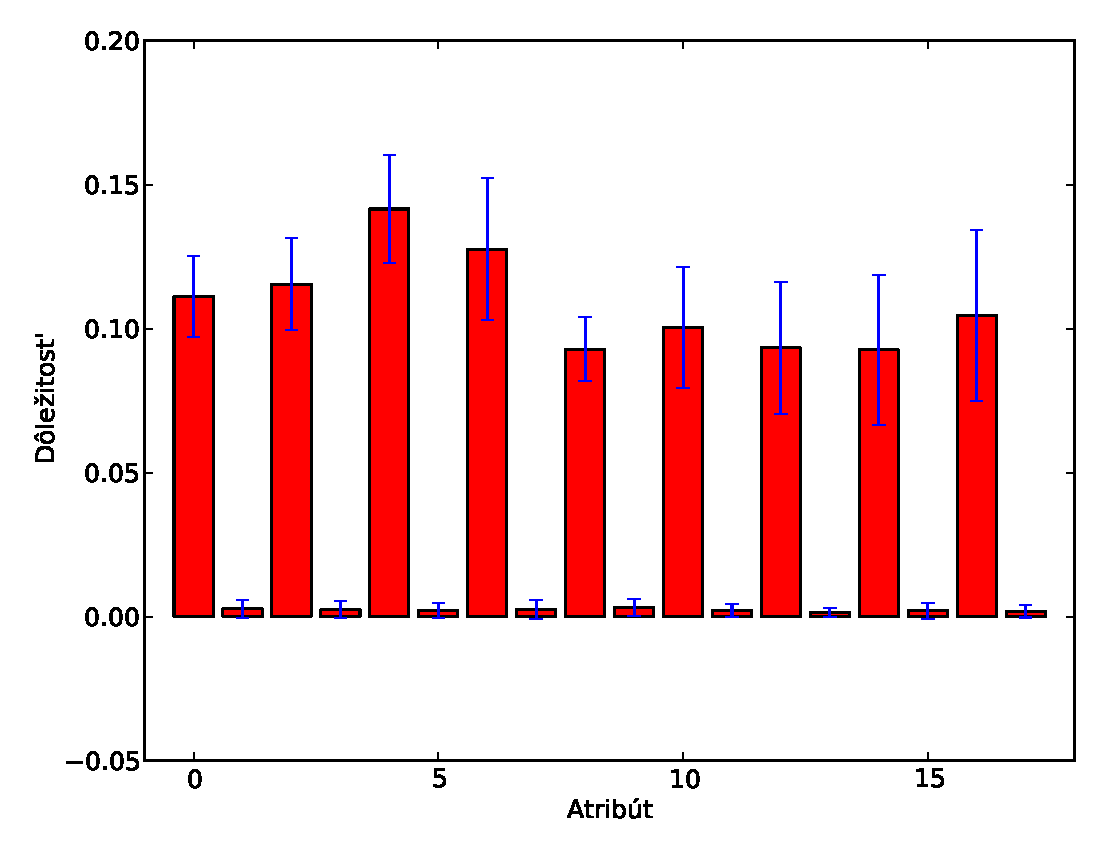
\includegraphics[width=\textwidth]{images/clf_fi/randomforest5_indel_bars}
                \includegraphics[width=\textwidth]{images/clf_fi/randomforest5_indel_heatmap}
                \caption{InDel klasifikátor}
                \label{fig:datatype1-i}
        \end{subfigure}
        \caption[Dôležitosť atribútov pre typ dát č. 1]{
        \textbf{Dôležitosť atribútov pre typ dát č. 1} - hodnoty sú normalizované aby súčet bol 1, modrý pásik označuje štandardnú odchýlku cez jednotlivé stromy v Random foreste.
        Pod grafom je tepelná mapa pre lepšiu vizualizáciu. Okno je veľkosti 5, takže aktuálne sa pýtame na 3tie pozície v okne t.j. bázy $x_3$, $y_3$ a ich anotácie $ax_3$ $ay_3$ (resp. v InDel klasifikátore len bázu $x_3$ a anotáciu $ax_3$)
        Atribúty v Match klasifikátore sú číslované nasledovne:\\
        \begin{tabular}{c|cccccccccc}
            & 0 & 1 & 2 & 3 & 4 & 5 & 6 & 7 & 8 & 9\\
            \hline
            0 & $x_1$ & $ax_1$ & $x_2$ & $ax_2$ & $x_3$ & $ax_3$ & $x_4$ & $ax_4$ & $x_5$ & $ax_5$\\
            1 & $y_1$ & $ay_1$ & $y_2$ & $ay_2$ & $y_3$ & $ay_3$ & $y_4$ & $ay_4$ & $y_5$ & $ay_5$
        \end{tabular}\\
        Atribúty v InDel klasifikátore sú číslované nasledovne:\\
        \begin{tabular}{c|cccccccccc}
            & 0 & 1 & 2 & 3 & 4 & 5 & 6 & 7 & 8 & 9\\
            \hline
            0 & $x_1$ & $ax_1$ & $x_2$ & $ax_2$ & $x_3$ & $ax_3$ & $x_4$ & $ax_4$ & $x_5$ & $ax_5$\\
            1 & $y_1$ & $ay_1$ & $y_2$ & $ay_2$ & $y_3$ & $ay_3$ & $y_4$ & $ay_4$ & &
        \end{tabular}\\
        pričom v tepelnej mape sú bázy a anotácie 3 a 4 posunuté doprava a medzi ne je vsunutá medzera.
        }
        \label{fig:datatype1}

\end{figure}

%m: .550822726889
%i: .32589867845

\subsection{Typ dát č. 2 - zhody v stĺpcoch okna}
\label{subsec:datatype2}

Druhý typ dát obsahuje aktuálnu bázu spolu s jej anotáciami a navyše pole veľkosti $k*w$, ktoré má na $i$-tom mieste 1 ak $okno_X[i] = okno_Y[i]$, ináč 0, pričom $w$ je veľkosť okna, $k$ je veľkosť bloku, $okno_X$ je časť okna zodpovedajúca $X$ sekvencii a $okno_Y$ zodpovedá $Y$-ovej časti okna.

Pri tomto type dát sa podľa obrázku \ref{fig:datatype2-m} Match klasifikátor najviac zameral na zhodu v bázach v centre okna potom v susedných a nakoniec na krajných bázach zhody v anotáciach mu neprišli vôbec dôležité.
Toto zodpovedá aj našej intuitívnej predstave o dôležitosti daných pozícií, akurát sme očakávali trochu väčšie zapojenie anotácií.
InDel klasifikátor podľa obrázku \ref{fig:datatype2-i} považoval za najdôležitejšie zhody v bázach na v ľavej časti, ďalej považoval za dôležité aj aktuálnu bázu a hlavne jej anotáciu, potom ostatné bázy.

\begin{figure}[htp]
        \centering
        \begin{subfigure}[t]{0.4\textwidth}
                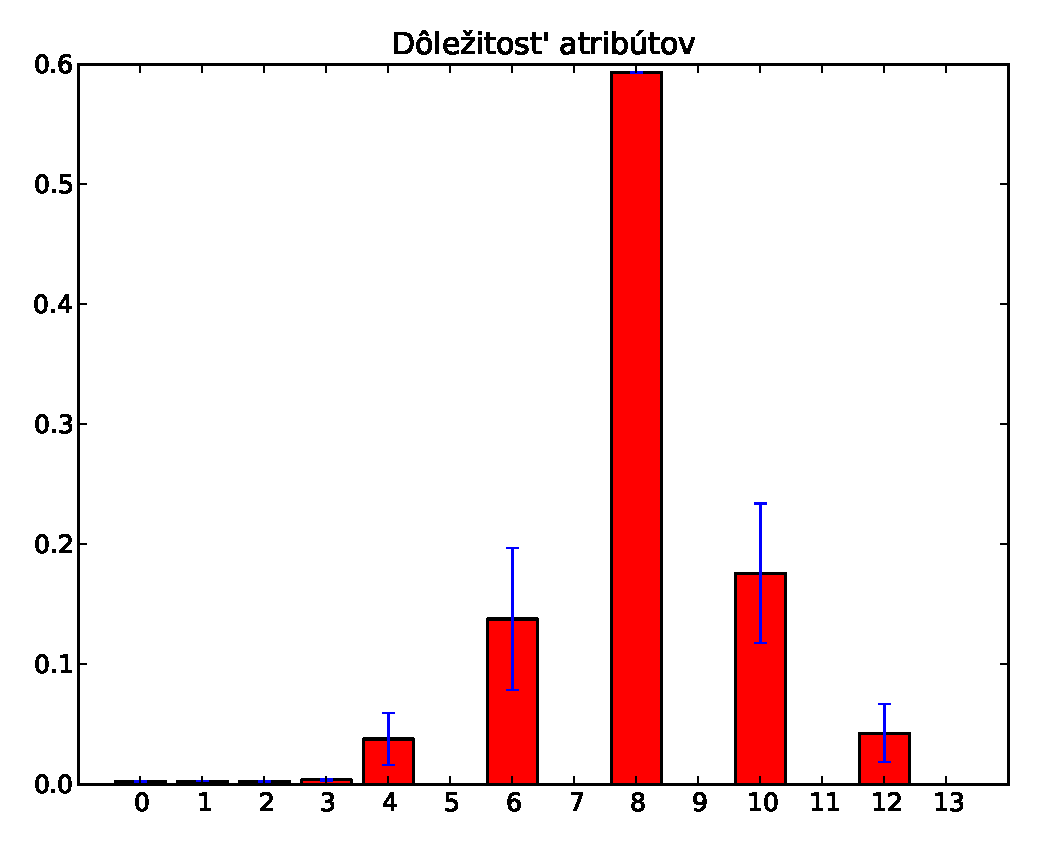
\includegraphics[width=\textwidth]{images/clf_fi/randomforest_cmp_5_bars}
                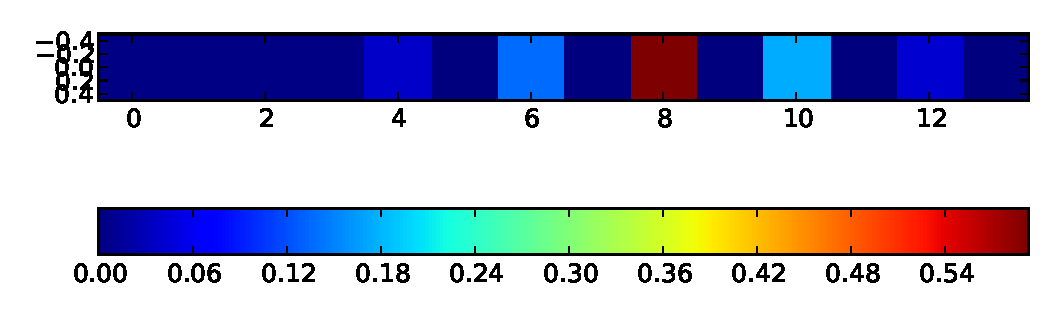
\includegraphics[width=\textwidth]{images/clf_fi/randomforest_cmp_5_heatmap}
                \caption{Match klasifikátor}
                \label{fig:datatype2-m}
        \end{subfigure}%
        \qquad\qquad %add desired spacing between images, e. g. ~, \quad, \qquad etc.
          %(or a blank line to force the subfigure onto a new line)
        \begin{subfigure}[t]{0.4\textwidth}
                \includegraphics[width=\textwidth]{images/clf_fi/randomforest_cmp_5_indel_bars}
                \includegraphics[width=\textwidth]{images/clf_fi/randomforest_cmp_5_indel_heatmap}
                \caption{InDel klasifikátor}
                \label{fig:datatype2-i}
        \end{subfigure}
        \caption[Dôležitosť atribútov pre typ dát č. 2]{
        \textbf{Dôležitosť atribútov pre typ dát č. 2} - hodnoty sú normalizované aby súčet bol 1, modrý pásik označuje štandardnú odchýlku cez jednotlivé stromy v Random foreste.
        Pod grafom je tepelná mapa pre lepšiu vizualizáciu. Okno je veľkosti 5. Bázy a anotácie na ktoré sa pýtame sú na začiatku - pozície 0-3 (resp. v InDel klasifikátore pozície 0-1)
        }
        \label{fig:datatype2}

\end{figure}

% .579200774008
% .275390935108

\subsection{Typ dát č. 3 - matica zhód v okne}

Tretí typ dát je podobný ako typ č. 2 (sekcia \ref{subsec:datatype2}), rozdiel je v tom, že teraz pole obsahuje nie len zhody po dvojiciach ale celú maticu zhôd. Teda opäť máme aktuálne bázy s anotáciami a pole má veľkosť $k*w^2$. Každý riadok sa skladá s jednotlivých blokov a v tabuľke v $x$-tom riadku, $y$-tom stĺpci a $i$-tom mieste v bloku je 1 práve
vtedy keď $okno_X[x+i] = okno_Y[y+i]$.

Keďže v tomto prípade máme veľa atribútov na vyhodnotenie okrem obrázka \ref{fig:datatype3}, ktorý nie je dostatočne prehľadný, pomôžeme aj tabuľkou \ref{tab:datatype3}.
\begin{table}[htp]
\centering
\begin{subtable}{\textwidth}
\centering
\begin{tabular}{r|cccc}
Poradie & atribút & dôležitosť & pozície v sekvencii (x, y) & báza/anotácia\\
\hline
1. & 41 & 0.355299 & (3, 3) & anotácia\\
2. & 52 & 0.236935 & (4, 4) & báza\\
3. & 17 & 0.121699 & (1, 1) & anotácia\\
4. & 28 & 0.116403 & (2, 2) & báza\\
5. & 4 & 0.097338 & (0, 0) & báza\\
\end{tabular}
\caption{Match klasifikátor}
\end{subtable}

\begin{subtable}{\textwidth}
\centering
\begin{tabular}{r|cccc}
Poradie & atribút & dôležitosť & pozície v sekvencii (x, y) & báza/anotácia\\
\hline
1. & 33 & 0.593272 & (3, 3) & anotácia\\
2. & 2 & 0.150084 & (0, 0) & báza\\
3. & 13 & 0.111226 & (1, 1) & anotácia\\
4. & 22 & 0.067791 & (2, 2) & báza\\
5. & 1 & 0.031562 & x:3 & anotácia\\
\end{tabular}
\caption{Indel klasifikátor}
\end{subtable}
\caption[Najdôležitejšie atribúty pre typ dát č. 3]{Najdôležitejšie atribúty pre typ dát č. 3}
\label{tab:datatype3}
\end{table}
Všimnime si, že najdôležitejšie atribúty sú na uhlopriečke, opäť zoradené podľa vzdialenosti od stredu, čo by zodpovedalo typu dát č. 1 (sekcia \ref{subsec:datatype1}), ibaže v tomto prípade sa nám vyskytli na niektorých pozíciách anotácie namiesto báz.
Avšak ak sa nám tam vyskytla anotácia, bázu už klasifikátor nepovažoval za dôležitú a aj naopak.
Indel klasifikátor navyše považoval za dôležitejšiu aj anotáciu na aktuálnej pozícii.

\begin{figure}[htp]
        \centering
        \begin{subfigure}[t]{0.4\textwidth}
                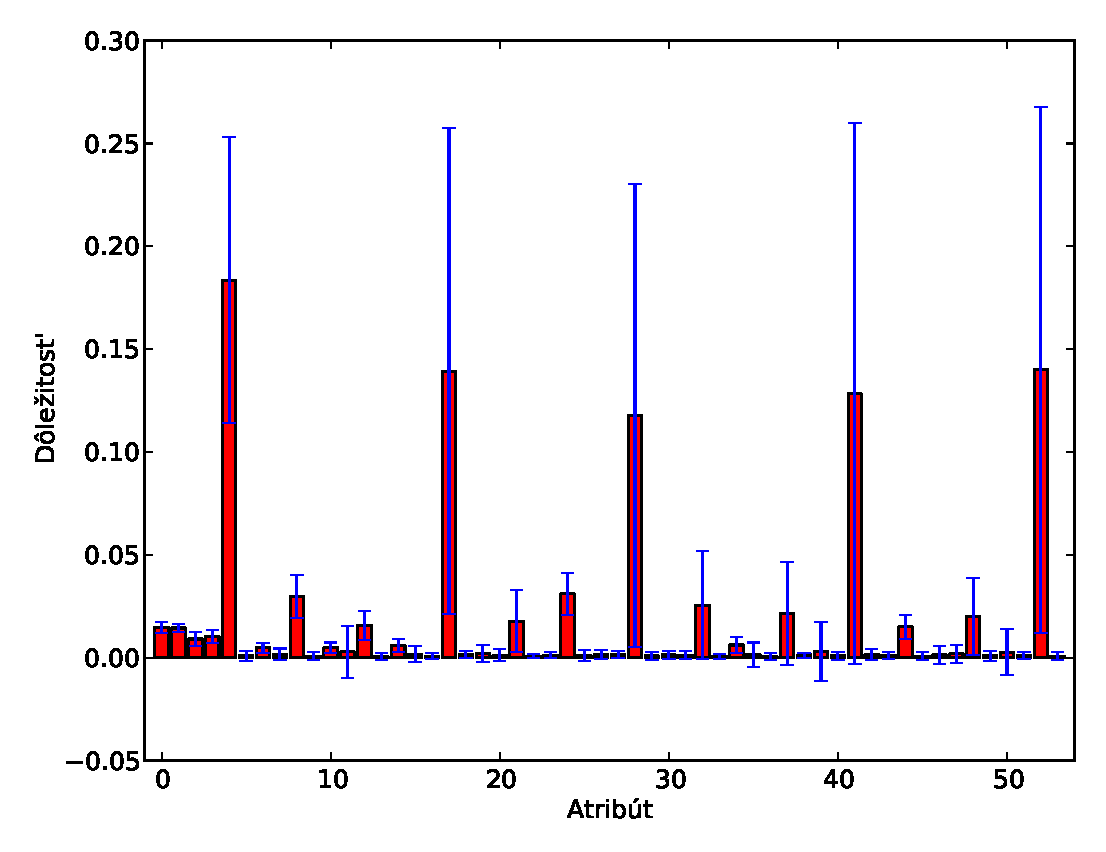
\includegraphics[width=\textwidth]{images/clf_fi/randomforest_fullcmp_5_bars}
                \includegraphics[width=\textwidth]{images/clf_fi/randomforest_fullcmp_5_heatmap}
                \caption{Match klasifikátor}
                \label{fig:datatype3-m}
        \end{subfigure}%
        \qquad\qquad %add desired spacing between images, e. g. ~, \quad, \qquad etc.
          %(or a blank line to force the subfigure onto a new line)
        \begin{subfigure}[t]{0.4\textwidth}
                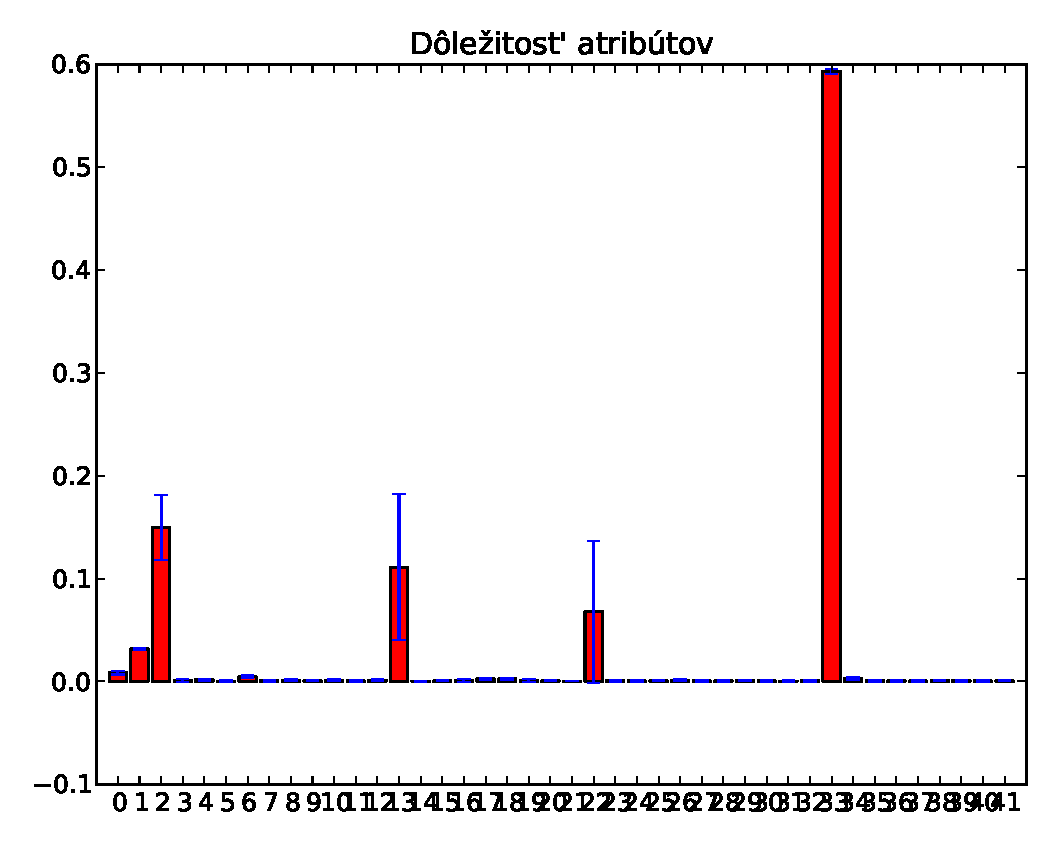
\includegraphics[width=\textwidth]{images/clf_fi/randomforest_fullcmp_5_indel_bars}
                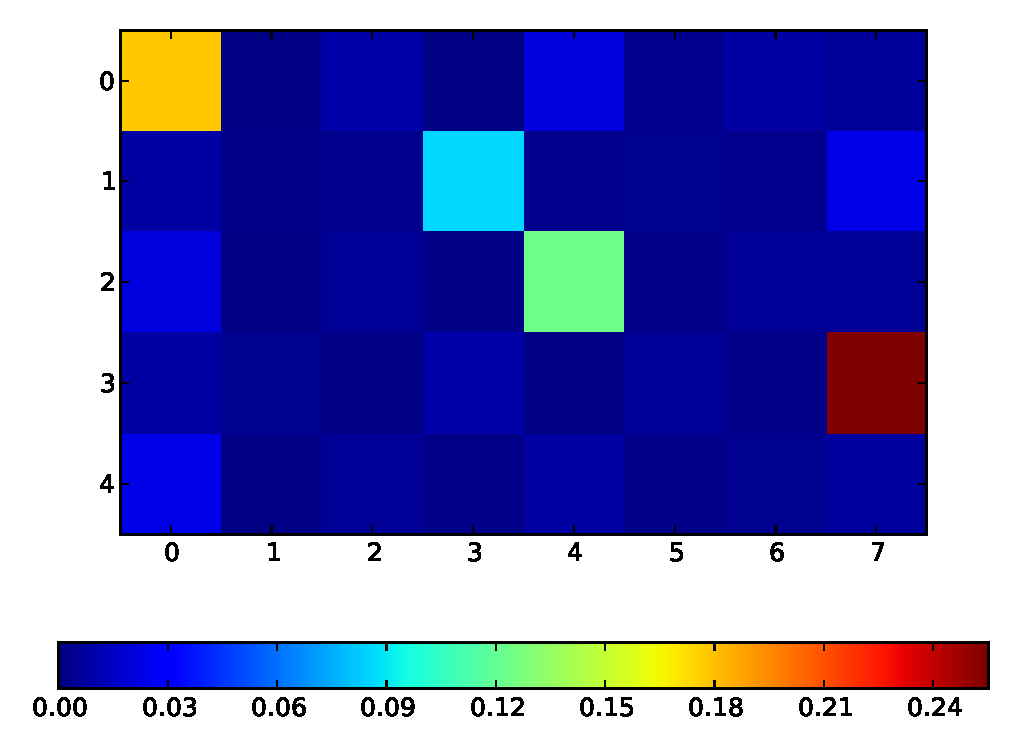
\includegraphics[width=\textwidth]{images/clf_fi/randomforest_fullcmp_5_indel_heatmap}
                \caption{InDel klasifikátor}
                \label{fig:datatype3-i}
        \end{subfigure}
        \caption[Dôležitosť atribútov pre typ dát č. 3]{
        \textbf{Dôležitosť atribútov pre typ dát č. 3} - hodnoty sú normalizované aby súčet bol 1, modrý pásik označuje štandardnú odchýlku cez jednotlivé stromy v Random foreste.
        Pod grafom je tepelná mapa pre lepšiu vizualizáciu. Bázy na ktoré sa pýtame sa spolu s anotáciami nachádajú na začiatku -- pozície 0-3 (resp. 0-1 v Indel klasifikátore) a v tepelnej mape sme ich pre prehľadnosť vynechali.
        V indel klasifikátore samozrejme chýba stredná pozícia v $y$-ovej sekvencii.
        }
        \label{fig:datatype3}

\end{figure}

%  .478942906979
%  .324760455914

\subsection{Typ dát č. 4 - kombinácia 1 a 2}

Posledný typ dát je kombináciou typov dát 1 a 2 (popísaných v sekciách \ref{subsec:datatype1} a \ref{subsec:datatype2}). Dáta opäť obsahujú všetky bázy a anotácie a navyše sme pridali pole zhód z dát typu 2. Táto informácia je síce redundantná a klasifikátor by si ju mal vedieť odvodiť aj sám, no predošlé experimenty ukázali, že by to mohlo pomôcť.

Na obrázku \label{fig:datatype4} si móžme všimnúť, že klasifikátory silno uprednostnili dáta typu 2 oproti dátam typu 1. Pohľad na konkrétne čísla nám prezradil, že pri Match klasifikátore najmenej zavážili zhody v anotáciách teda dáta typu 1 boli zrejme pre klasifikátor užitočné na nejaké jemnejšie delenie.
Pri InDel klasifikátore si môžme všimnúť, že aj ostatné dáta mali nezanedbateľnú dôležitosť.

\begin{figure}[htp]
        \centering
        \begin{subfigure}[t]{0.4\textwidth}
                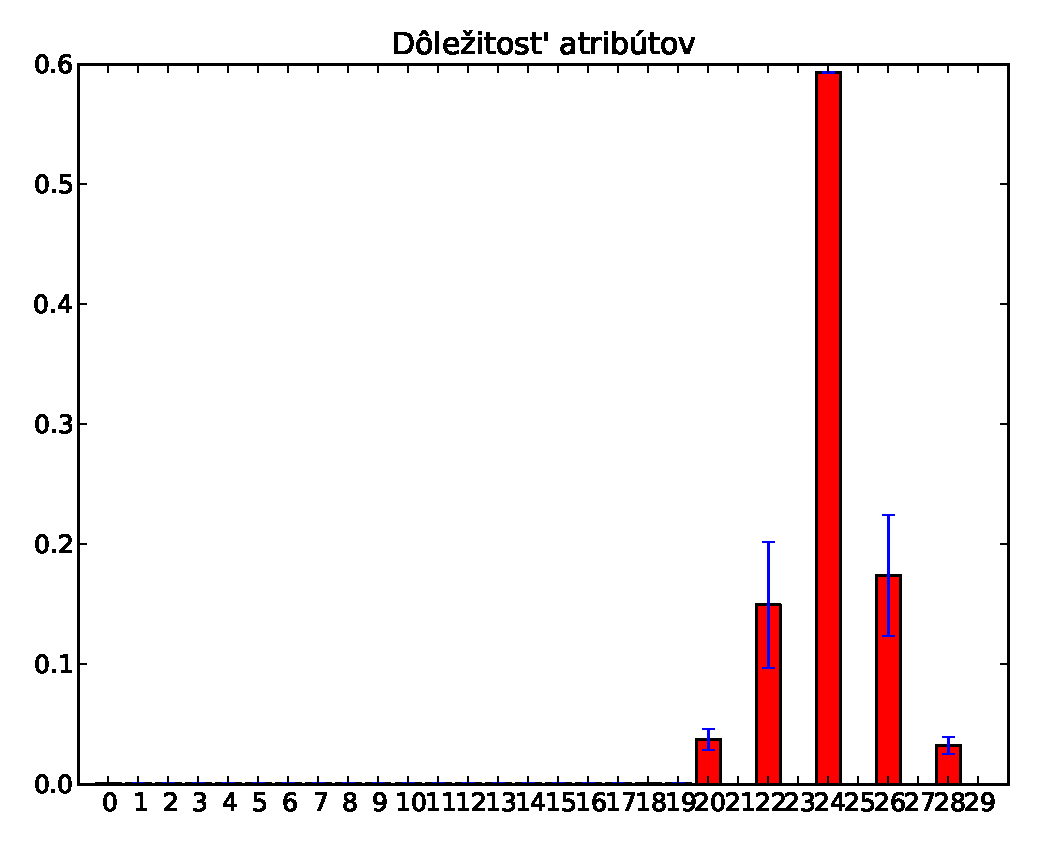
\includegraphics[width=\textwidth]{images/clf_fi/randomforest_combined_5_bars}
                \includegraphics[width=\textwidth]{images/clf_fi/randomforest_combined_5_heatmap}
                \caption{Match klasifikátor}
                \label{fig:datatype4-m}
        \end{subfigure}%
        \qquad\qquad %add desired spacing between images, e. g. ~, \quad, \qquad etc.
          %(or a blank line to force the subfigure onto a new line)
        \begin{subfigure}[t]{0.4\textwidth}
                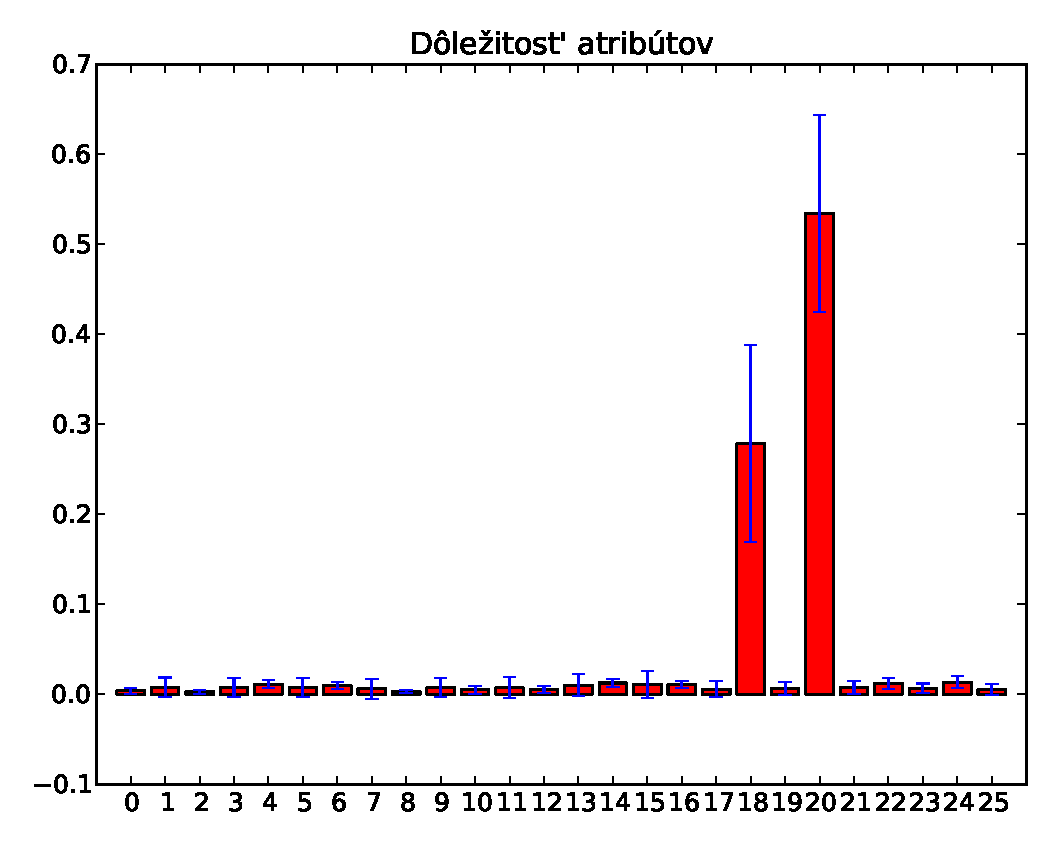
\includegraphics[width=\textwidth]{images/clf_fi/randomforest_combined_5_indel_bars}
                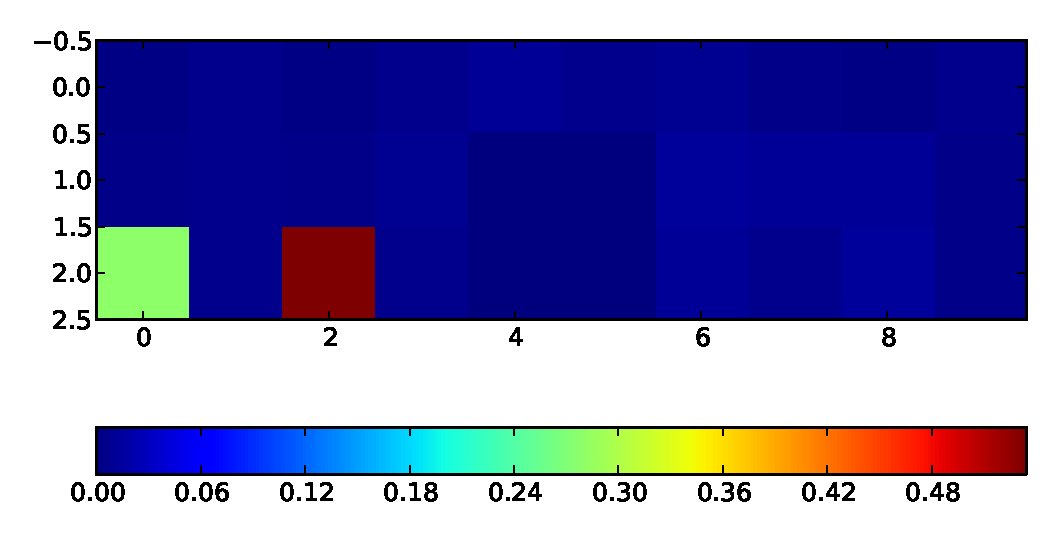
\includegraphics[width=\textwidth]{images/clf_fi/randomforest_combined_5_indel_heatmap}
                \caption{InDel klasifikátor}
                \label{fig:datatype2-i}
        \end{subfigure}
        \caption[Dôležitosť atribútov pre typ dát č. 4]{
        \textbf{Dôležitosť atribútov pre typ dát č. 4} - hodnoty sú normalizované aby súčet bol 1, modrý pásik označuje štandardnú odchýlku cez jednotlivé stromy v Random foreste.
        Pod grafom je tepelná mapa pre lepšiu vizualizáciu. Okno je veľkosti 5, takže aktuálne sa pýtame na 3tie pozície v okne t.j. bázy $x_3$, $y_3$ a ich anotácie $ax_3$ $ay_3$ (resp. v InDel klasifikátore len bázu $x_3$ a anotáciu $ax_3$)
        }
        \label{fig:datatype4}

\end{figure}

% .574262060724
% .378158256744

\subsection{Zhrnutie}

\todo ktorý typ dát sa nám zdal najvhodnejší a prečo



\begin{table}[htp]
\centering
\begin{tabular}{r|cc}
Typ dát & Match & Indel\\
\hline
1 & 55,08\% & 32,59\%\\
2 & 57,92\% & 27,54\%\\
3 & 47,89\% & 32,48\%\\
4 & 57,43\% & 37,82\%\\
\end{tabular}
\caption[Úspešnosť klasifikátorov pri rôznych typoch dát]{Úspešnosť Match a Indel klasifikátorov pri rôznych spôspboch predspracovania dát}
\label{tab:datatype3}
\end{table}

\section{Trénovanie}

\subsection{Výber pozitívnych a negatívnych príkladov pre Match klasifikátor}

\subsection{Výber pozitívnych a negatívnych príkladov pre Indel klasifikátor}

% \section{Random Forest}

% \todo chcem to tu, alebo niekde inde?

% \todo



